\subsection{Analyse der blauen $\sigma$-Linien}
Vollkommen analog wird die $\sigma$-Aufspaltung des blauen Lichtes analysiert.
Die Aufspaltung der blauen Spektrallinie ist in Abbildung \ref{fig: aufspaltung_blau_sigma} dargestellt.
Gemäß Formel \eqref{eq: fitfuntion_hysterese}
führt der anliegende Spulenstrom von $I = \SI{10}{\ampere}$ zu einer magnetischen Feldstärke von $B = \SI{346(3)}{\milli\tesla}$.
\begin{figure}
  \centering
  \includegraphics[width = 0.7\textwidth]{../Messdaten/bilder_v27/messung_2_blau_sigma/aufspaltung_blau_sigma.png}
  \caption{Blau $\sigma$: Aufgenommene Intensitätsstreifen des blauen Lichtes (von oben nach unten) $\SI{0}{\ampere}$ und $\SI{6}{\ampere}$ Feldstrom.}
  \label{fig: aufspaltung_blau_sigma}
\end{figure}
Die Helligkeit in Abhängigkeit von der horizontalen Position auf den aufgenommenen Bildern ist in Abbildung \ref{fig: blau_intensität_sigma} für das unaufgespaltene
und aufgespaltene Beugungsbild dargestellt. Anhand dessen werden die Positionen von $10$ Intensitätsmaxima und ihrer Aufspaltungen
vermessen. Die Daten sind in Tabelle \ref{tab: peaks_blau_sigma} aufgeführt.
\begin{figure}
  \centering
  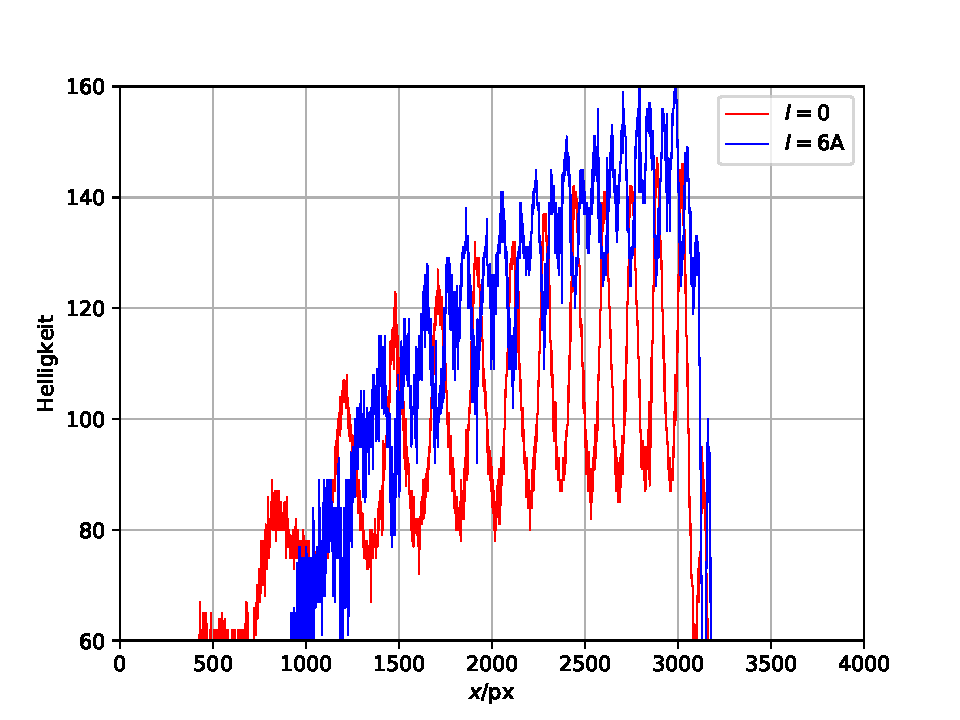
\includegraphics[width = 0.7\textwidth]{../Messdaten/plots/blau_sigma_intensitaet.pdf}
  \caption{Blau $\sigma$: Darstellung der Helligkeit der blauen Linien in Abhängigkeit von der horizontalen Lage auf dem Foto.}
  \label{fig: blau_intensität_sigma}
\end{figure}
\begin{table}
\centering
\caption{Blaue Sigma Aufspaltung: Positionen $x_0$ und $x_{6}$ der Intensitätsmaxima unter $I= \SI{0}{\ampere}$ und $I= \SI{6}{\ampere}$.}
\label{tab: peaks_blau_sigma}
\begin{tabular}{S S[table-format=4.0] S[table-format=4.0] } 
\toprule
{$x_0 / $px} & \multicolumn{2}{c}{$x_{6} \:/\: $px} \\
\midrule
1483 & 1408 & 2402\\
1708 & 1539 & 2487\\
1909 & 1641 & 2555\\
2121 & 1759 & 2641\\
2285 & 1859 & 2702\\
2449 & 1967 & 2788\\
2605 & 2051 & 2843\\
2752 & 2154 & 2930\\
2891 & 2235 & 2985\\
3030 & 2320 & 3052\\
\bottomrule
\end{tabular}
\end{table}

Eine graphische Darstellung der abgelesenen Intensitätsmaxima befindet sich in den Abbildungen \ref{fig: peaks_blau_0} und \ref{fig: peaks_blau_sigma_6}.
\begin{figure}
  \centering
  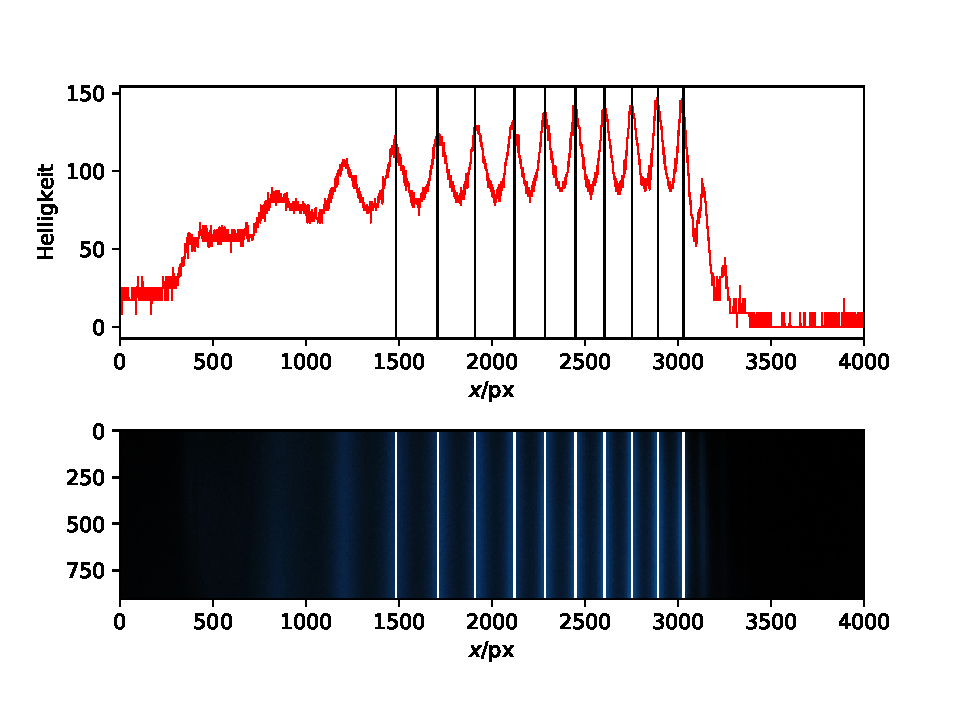
\includegraphics[width = 0.7\textwidth]{../Messdaten/plots/peaks_blau_sigma_0.pdf}
  \caption{Darstellung der abgelesenen Lagen der Intesitätsmaxima für das Beugungsbild unter $I =0$A.}
  \label{fig: peaks_blau_0}
\end{figure}
\begin{figure}
  \centering
  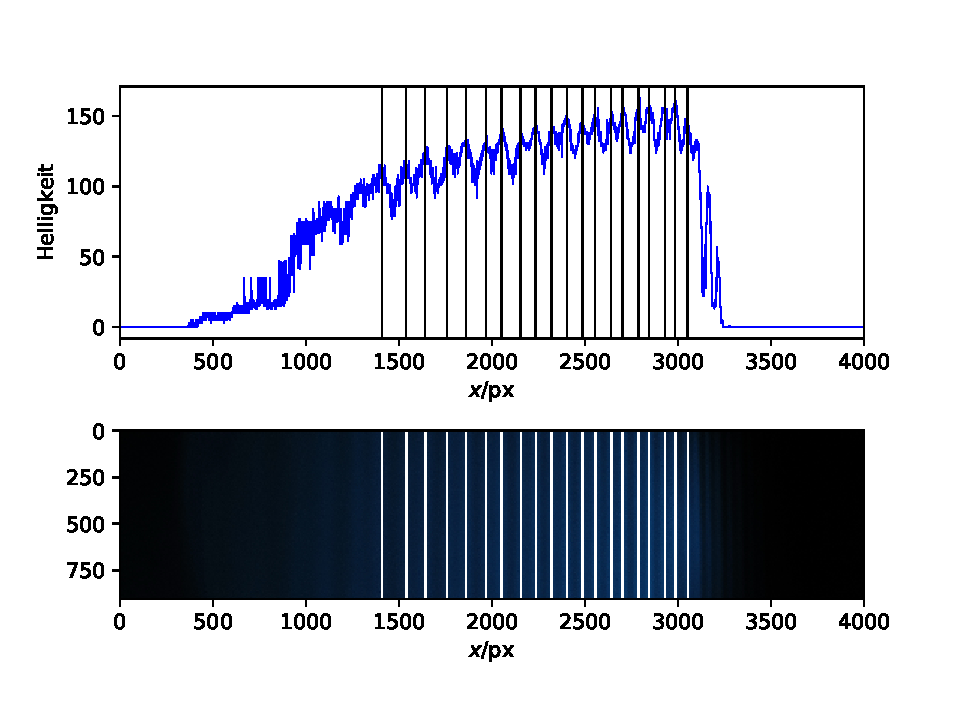
\includegraphics[width = 0.7\textwidth]{../Messdaten/plots/peaks_blau_sigma_6.pdf}
  \caption{Blau $\sigma$: Darstellung der abgelesenen Lagen der Intesitätsmaxima für das Beugungsbild unter $I =6$A.}
  \label{fig: peaks_blau_sigma_6}
\end{figure}
Die für die Berechnung der Wellenlängenänderung relevanten Abstände $\Delta s_i$ und $\delta s_i$ sind in Tabelle \ref{tab: abstände_blau_sigma}
aufgeführt. Mit Hilfe der Gleichungen \eqref{} berechneten Größen sind in Tabelle
\ref{tab: abstände_blau_sigma} eingetragen. Als Mittelwert für den Landé-Faktor ergibt sich
\begin{equation}
  g = \num{2.02(2)}.
\end{equation}
\input{../Messdaten/tabs/abstände_blau_sigma.tex}
